\documentclass[a4paper]{article}
\usepackage[utf8]{inputenc}
\usepackage[spanish, es-tabla, es-noshorthands]{babel}
\usepackage[table,xcdraw]{xcolor}
\usepackage[a4paper, footnotesep = 1cm, width=20cm, top=2.5cm, height=25cm, textwidth=18cm, textheight=25cm]{geometry}
%\geometry{showframe}

\usepackage{tikz}
\usepackage{amsmath}
\usepackage{amsfonts}
\usepackage{amssymb}
\usepackage{float}
\usepackage{graphicx}
\usepackage{caption}
\usepackage{subcaption}
\usepackage{multicol}
\usepackage{multirow}
\setlength{\doublerulesep}{\arrayrulewidth}
\usepackage{booktabs}

\usepackage{hyperref}
\hypersetup{
    colorlinks=true,
    linkcolor=blue,
    filecolor=magenta,      
    urlcolor=blue,
    citecolor=blue,    
}

\newcommand{\quotes}[1]{``#1''}
\usepackage{array}
\newcolumntype{C}[1]{>{\centering\let\newline\\\arraybackslash\hspace{0pt}}m{#1}}
\usepackage[american]{circuitikz}
\usetikzlibrary{calc}
\usepackage{fancyhdr}
\usepackage{units} 

\graphicspath{{../Ejercicio-1/}{../Ejercicio-2/}{../Ejercicio-3/}{../Ejercicio-4/}}

\pagestyle{fancy}
\fancyhf{}
\lhead{22.01 Teoría de Circuitos}
\rhead{Mechoulam, Lambertucci, Rodriguez Turco, Londero, Galdeman}
\rfoot{\centering \thepage}

\begin{document}
\subsection{Análisis Cualitativo del Circuito Base}

El siguiente análisis no cuantitativo del circuito base se comprobará más adelante a la hora de realizar las simulaciones y el subsiguiente prototipeado.

\subsubsection{Etapa de Alimentación}

La alimentación del circuito es una fuente no partida de $9V$. Se observa que el capacitor electrolítico $C_5$ se encuentra justo a la salida de la fuente de alimentación. Se presume que la utilidad de este es para filtrar cualquier ruido que haya montado sobre la continua, ya que por su conexión a tierra, cualquier tensión no contante encontrará un camino de baja impedancia hacia masa.

\begin{figure}[H]
	\centering
	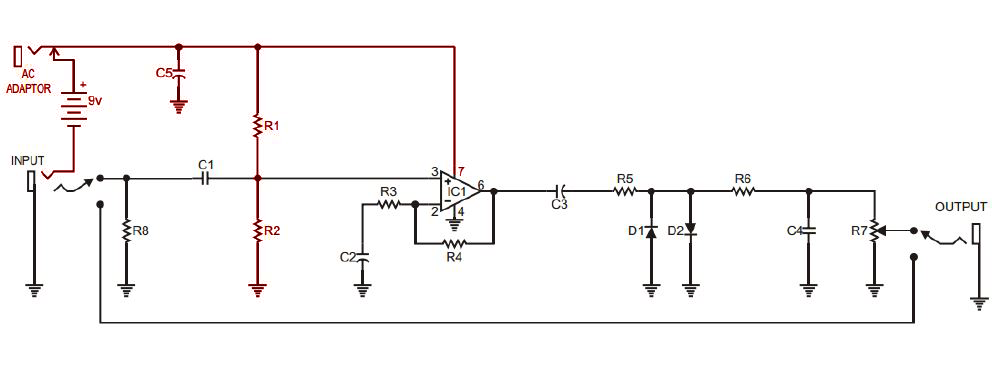
\includegraphics[width=1\textwidth, trim={0 0 0 0}, clip]{Ejercicio5/Imagenes/circuito_base_alimentacion.png}
	\caption{Alimentación del circuito base.}
	\label{fig:circuito_base_alimentacion}
\end{figure}

Luego pueden verse dos resistencias $R_1$ y $R_2$, donde $R_1$ está conectada a la señal de entrada y $R_2$ está conectada a la resistencia anterior y a tierra. Este par puede considerarse de manera aproximada como un divisor resistivo, ya que en el punto medio se ofrece gran impedancia por parte tanto del op-amp (despreciando la corriente de entrada) como por el capacitor $C_1$, ya que la tensión de alimentación es constante.
Este divisor resistivo lo que está haciendo es montando a la señal de entrada sobre la tensión en el punto medio. Es en este punto donde se soluciona el problema de tener una sola fuente no partida ya que, si se cumple que $R_1=R_2$, la señal de entrada quedará levantada $4.5V$, por lo que se podría alimentar al op-amp solo de manera positiva, llevando a tierra la alimentación negativa.\\

Por último, se llevan los $9V$ de la fuente de alimentación a la entrada de alimentación positiva del op-amp.


\subsubsection{Etapa de Pre-amplificación}

\begin{figure}[H]
	\centering
	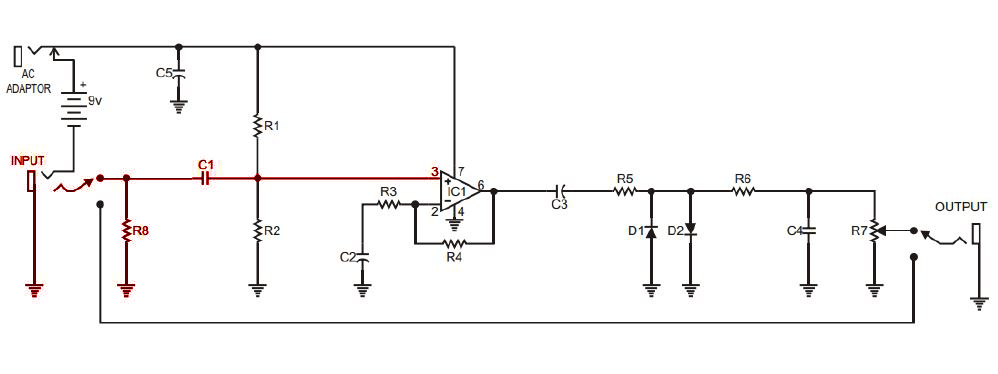
\includegraphics[width=1\textwidth, trim={0 0 0 0}, clip]{Ejercicio5/Imagenes/circuito_base_preamplificacion.png}
	\caption{Etapa de pre-amplificación del circuito base.}
	\label{fig:circuito_base_preamplificacion}
\end{figure}

Justo luego de la entrada se encuentra la resistencia $R_8$. Esta resistencia podría situarse en este lugar para atenuar levemente la entrada y ayudar a filtrar pequeños picos muy rápidos de tensión en la entrada. Otra hipótesis es que ayuda a elevar la impedancia de entrada de todo el circuito.\\

El capacitor $C_1$, como ya dicho antes, ofrece gran impedancia a la tensión continua de la alimentación para proteger a la entrada. De otra manera, la señal continua ingresaría por la entrada.
Lo que se obtiene posterior al capacitor será la señal de entrada levantada tantos voltios como proporcionen el punto medio del divisor resistivo.\\

Se contempla además que el circuito base nos permite tener una opción de realizar un bypass total al circuito mediante el uso de una llave.

\subsubsection{Etapa de Amplificación}

El operacional se encuentra realimentado negativamente con una configuración no inversora. No es un problema que no este alimentado negativamente, ya que la señal de entrada estará montada sobre una continua.

\begin{figure}[H]
	\centering
	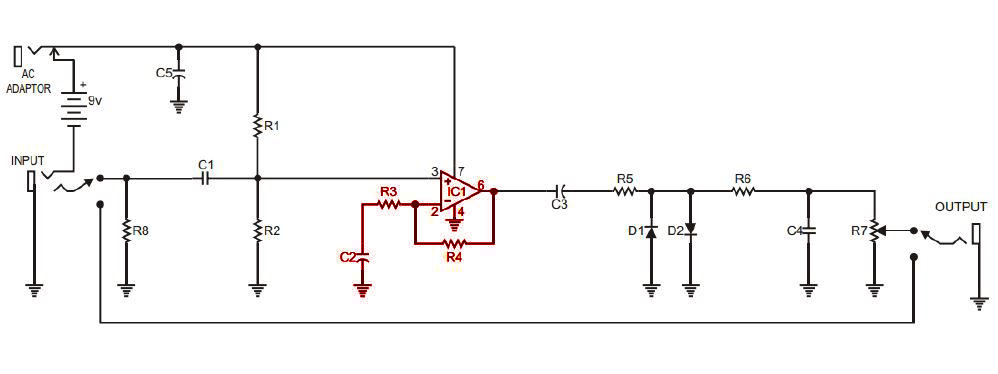
\includegraphics[width=1\textwidth, trim={0 0 0 0}, clip]{Ejercicio5/Imagenes/circuito_base_amplificacion.png}
	\caption{Etapa de amplificación del circuito base.}
	\label{fig:circuito_base_amplificacion}
\end{figure}

Analizando el lazo del op-amp, se puede observar que la realimentación dependerá de la frecuencia. Esto puede observarse ya que para bajas frecuencias el capacitor actúa con gran impedancia, por lo que el operacional amplifica menos. Para las frecuencias altas el operacional amplificará cada vez más la señal hasta llegar al polo dominante. Sin embargo, lo mas importante del posicionamiento de este capacitor en el lazo de realimentación es que impide que el operacional amplifique la continua sobre la cual está montada la señal, ya que en este caso el capacitor se comporta como un circuito abierto. Esto hace que el operacional funcione como un seguidor de tensión, trabajando para fijar la continua de la salida en el mismo valor que la de la referencia. Se observa como es aquí, en el lazo de realimentación, donde se podría controlar la amplificacion de las distintas frecuencias por separado.

\subsubsection{Etapa de Ecualización}

A la salida del operacional se encuentra el capacitor $C_3$. Este capacitor se utiliza para remover la continua sobre la cual estaba montada la señal de entrada.

\begin{figure}[H]
	\centering
	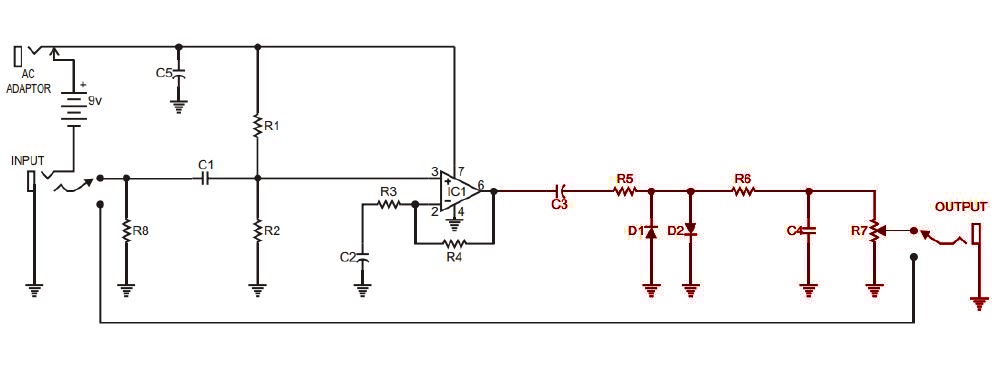
\includegraphics[width=1\textwidth, trim={0 0 0 0}, clip]{Ejercicio5/Imagenes/circuito_base_ecualizacion.png}
	\caption{Etapa de ecualización del circuito base.}
	\label{fig:circuito_base_ecualizacion}
\end{figure}

Luego, se encuentra en el circuito una resistencia en serie con un par de diodos en paralelo con polaridad invertida. Estos diodos fijarían la tensión de la señal en $V_{d_{on}}$ tanto para el semi-ciclo positivo como para el negativo, deformando la señal generando un efecto de "clipping". La resistencia $R_5$ limita la corriente de los diodos. Se presume que esto se apreciaría como una gran distorsión a la hora de conectar una guitarra y escuchar la salida.\\

Seguido de los diodos se puede encontrar un pequeño circuito R-C cuya finalidad podría ser la de darle un último cambio a la señal. Este circuito estaría posicionando un polo en la respuesta en frecuencia, atenuando las frecuencias altas. Se deberá comprobar mediante simulaciones y protobordeado el posible uso de este último tramo.

Finalmente antes de la salida se encuentra un potenciómetro, el cual se presume que se utiliza como control de volumen de salida.

\subsection{Análisis Cuantitativo del Circuito Base}

Tanto el análisis cuantitativo como el subsiguiente diseño de un nuevo circuito propuesto se harán a partir de lo estudiado en diversas fuentes de internet, como en el libro \textbf{PREGUNTAR NOMBRE DEL LIBRO DE AGUSTIN}.

Además, se decidió, para presentar lo realizado de la forma más clara, primero realizar un análisis teórico-analítico del circuito base para luego presentar sólamente los cambios propuestos.\\

\subsubsection{Componentes}

\textbf{$R_8$:} Se quiere que la impedancia de entrada al circuito sea mucho más grande que la impedancia de salida de una guitarra eléctrica con pick-ups normales, la cual es de aproximadamente $10 \ k\Omega$. Si la impedancia de entrada al circuito fuese del orden de la impedancia de salida de la guitarra, se cargarían los pick-ups y habría un desplazamiento de las frecuencias de resonancia y pérdida de agudos. Por esta razón, se decidió utilizar un valor de $1 \ M\Omega$ para este resistor. Luego en la sección de impedancia de entrada se repasara su efecto. \\

\textbf{$R_1$, $R_2$:} Se quiere montar a la señal de entrada sobre una continua de la mitad del valor que la de la alimentación, por esto, se decidió que $R_1=R_2$.

Se utilizaron valores relativamente grandes para las resistencias del divisor de tensión por dos razones:
\begin{itemize}
\item Que la corriente de stand-by no sea muy alta.
\item La resistencia $R_2$ contribuya a la impedancia de entrada total del circuito.
\end{itemize}
El valor utilizado es de $R_1=R_2=510 \ k\Omega$, con posibles cambios tras el simulado del circuito.\\

\textbf{$C_1$:} Como este capacitor filtra la continua provista por la alimentación, se decidió utilizar un valor de $10 \ nC$ ya que no se quiso que el efecto del filtro R-C que se forma con la resistencia $R_2$ se minimizara dentro de las frecuencias audibles ($20Hz-20kHz$).\\

\textbf{$C_5$:} Este capacitor filtrará las frecuencias de línea de $50Hz$, con un valor de $1nF$. \\

\textbf{$R_4, R_3$:} Se eligieron valores de $R_4=20R_3=1k$ para lograr una ganancia de aproximadamente $26,4 \ dB$.\\

\textbf{$C_2$:} Se quiso lograr una mayor amplificación de medios y agudos, por lo que el valor del capacitor fue fijado por la frecuencia de corte del filtro pasa-altos que se forma con la resistencia $R_3$. Este valor fue de $100nF$.\\

\textbf{$C_3$:} Este capacitor esta solamente para filtrar la continua de la salida del operacional, su valor será de $0.1\mu F$.\\

\textbf{$R_5, R_6$:} $R_5$ está para limitar la corriente de los diodos, se eligió un valor de $6k8\Omega$. $R_6$ formará un filtro pasabajos con $C_4$, eligió nuevamente un valor de $6k8\Omega$.\\

\textbf{$C_4$:} Se eligió un valor de $0.1\mu F$ para comenzar la simulación.\\

\textbf{$R_7$:} Este resistor será un potenciómetro logarítmico de $20k\Omega$. Logarítmico ya que de esta manera se acopla mejor a la escucha humana.

\subsubsection{Impedancia de Entrada}

Para un circuito con esta aplicación se quiere como ya dicho la mayor impedancia de entrada posible para no perder agudos o armónicos.
La impedancia de entrada del circuito base puede calcularse como
\[Z_{in} = R_8//(R_1//R_2)//Z_{in_{opamp}}\]
y deberá ser analizada por separado al momento de elegir un amplificador operacional.

\subsubsection{Impedancia de Salida}

La impedancia de salida se quiere mantener lo mas baja posible, ya que la impedancia de un parlante común ronda los $8\Omega$.
La impedancia de salida del circuito base puede calcularse como
\[ Z_{out} = Z_{out_{opamp}} + 6k8\Omega + 6k8\Omega \approx 13k6\Omega \]

\subsection{Simulación del Circuito Base}

Para realizar una primera simulación del circuito se utilizó el operacional LT1001. Se logró realizar
 
\end{document}